\documentclass[12pt,a4paper]{report}
\usepackage[utf8]{inputenc}
\usepackage[english,russian]{babel}
\usepackage{indentfirst}
\usepackage{pdfpages}
\usepackage{titlesec}
\usepackage{listings}
\usepackage{amsmath}

% Вставка картинки
\usepackage{graphicx}
\graphicspath{{schemes/}}
\DeclareGraphicsExtensions{.pdf,.png,.jpg}

\usepackage[14pt]{extsizes}

\newcommand{\hsp}{\hspace{20pt}}
\titleformat{\chapter}[hang]{\large\bfseries}{\thechapter{. }}{0pt}{\large\bfseries}
\titlelabel{hlabel-formati}
\titlespacing{\chapter}{42pt}{-20pt}{12pt}
\titleformat{\section}[hang]{\large\bfseries}{\thesection{. }}{0pt}{\large\bfseries}
\titlespacing{\section}{42pt}{12pt}{5pt plus 5pt}

% Отступ абзаца
\usepackage{indentfirst}
\setlength{\parindent}{1.5cm}

% Межстрочный интервал
\usepackage{setspace}
\onehalfspacing % интервал 1.5

\usepackage[left=3cm, right=1cm, top=2cm, bottom=2cm]{geometry}

\begin{document}
% Титульник
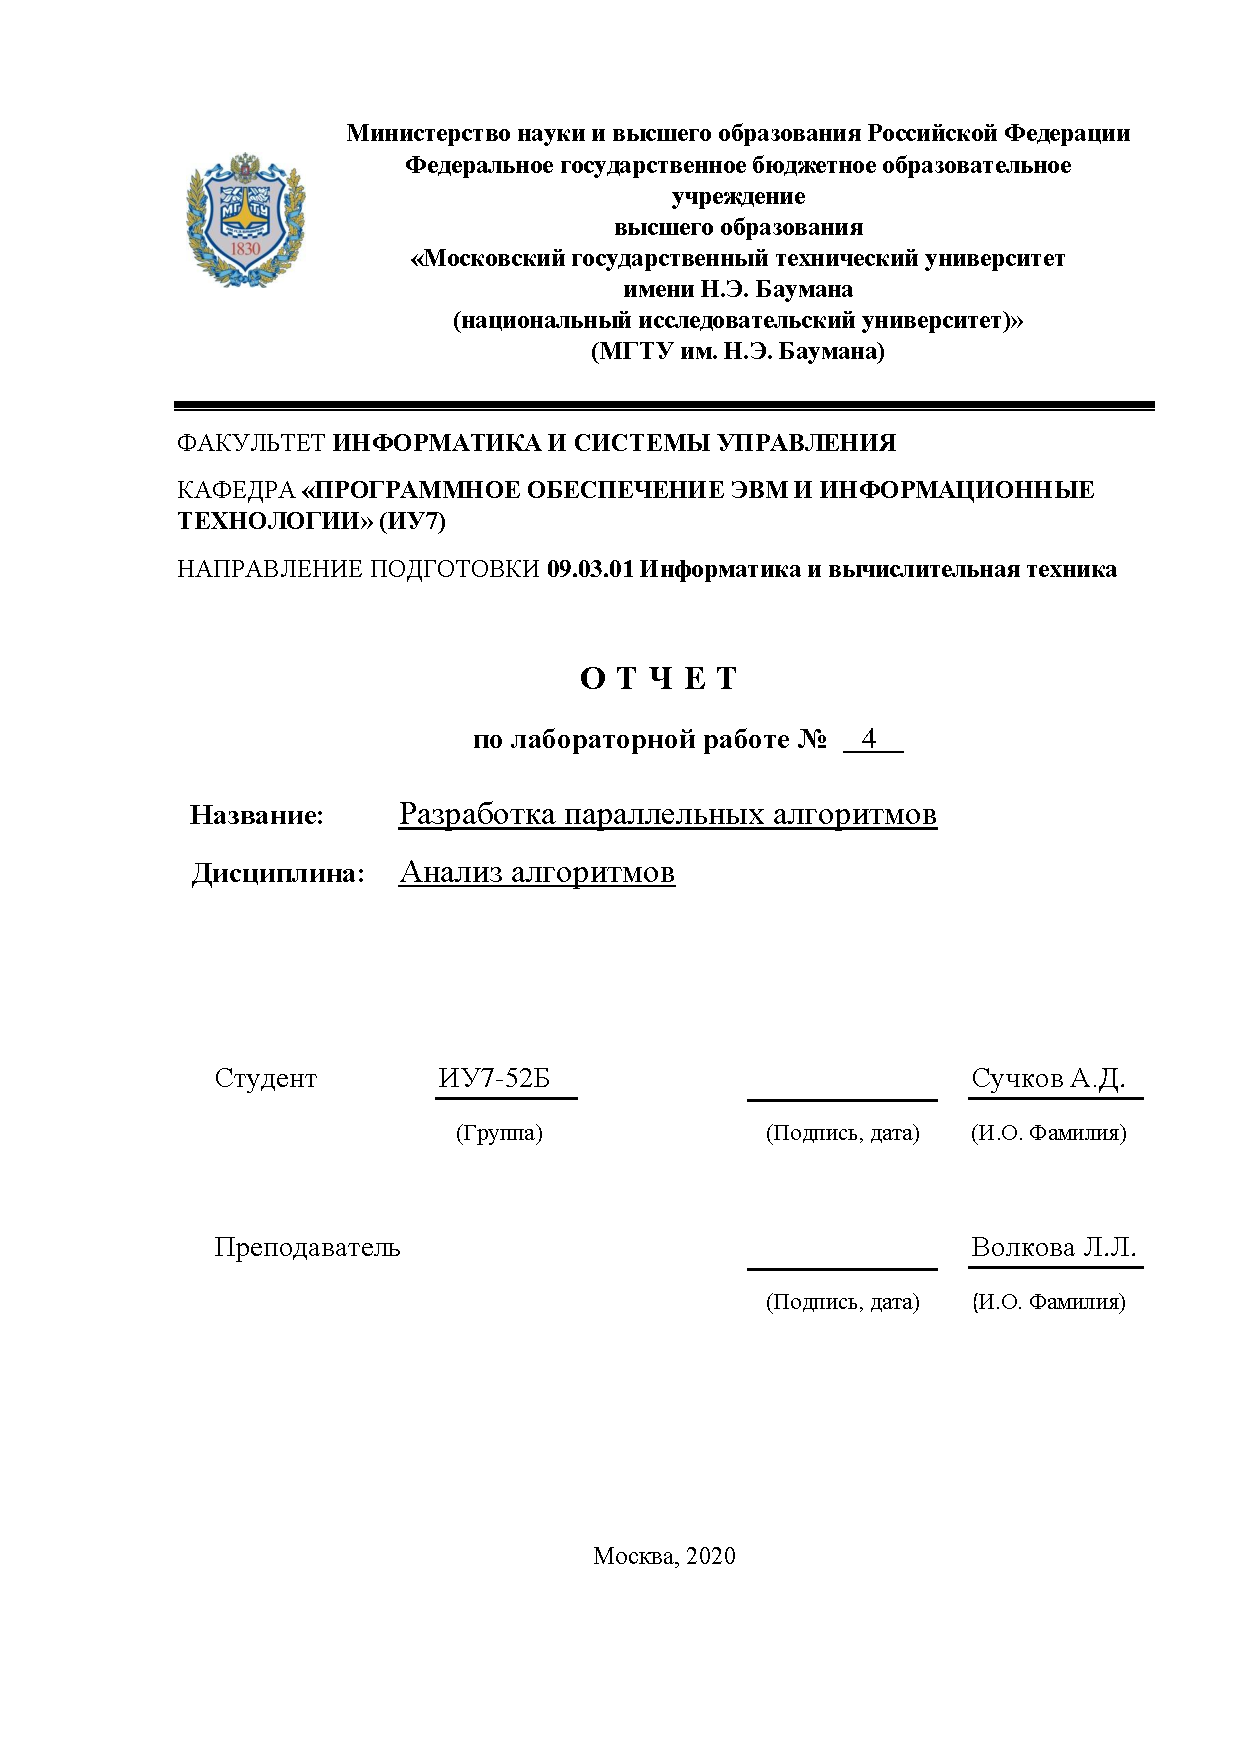
\includepdf[pages=1]{titul.pdf}
% Оглавление
\tableofcontents

\newpage
\chapter*{Введение}
\addcontentsline{toc}{chapter}{Введение}

\newpage
\chapter{Аналитическая часть}

\newpage
\chapter{Конструкторская часть}

\newpage
\chapter{Технологическая часть} 

\newpage
\chapter*{Заключение}
\addcontentsline{toc}{chapter}{Заключение}

\newpage
\renewcommand\bibname{Список литературы}
\addcontentsline{toc}{chapter}{Список литературы}
\makeatletter % список литературы
\def\@biblabel#1{#1. }
\makeatother
\begin{thebibliography}{2}
    \bibitem{analyse_info} Дж. Макконнел. Анализ алгоритмов. Активный обучающий подход. -- М.: Техносфера, 2017. -- 267с.
    \bibitem{time_bib} Документация на официальном сайте Python про библиотеку time [Электронный ресурс]. Режим доступа: https://docs.python.org/3/library/time.html (дата обращения 23.09.2020)
\end{thebibliography}

\end{document}

